
%% Creator David Li
% Modified matlab xsl latex template file to suit needs
% This LaTeX was auto-generated from an M-file by MATLAB.
% To make changes, update the M-file and republish this document.

\documentclass[12pt]{scrartcl}
\nonstopmode

\title{Matlab}
\usepackage[utf8]{inputenc}
\usepackage{graphicx}
\usepackage{epstopdf}
\usepackage{color}
\usepackage{xcolor}
\usepackage{amsmath}
\usepackage[ocgcolorlinks]{hyperref}
\usepackage{bookmark}
\usepackage[hmargin=2cm,vmargin=1.5cm]{geometry}
\usepackage{booktabs}
\sloppy
\definecolor{lightgray}{gray}{0.5}
% \definecolor{myText}{HTML}{2B2B2B}
\definecolor{fontColor}{HTML}{171717}
\setlength{\parindent}{0pt}

\makeindex

\usepackage{listings}
\definecolor{mygreen}{RGB}{28,172,0} % color values Red, Green, Blue
\definecolor{mylilas}{RGB}{170,55,241}
\lstset{language=Matlab,%
	%basicstyle=\color{red},
	breaklines=true,%
	morekeywords={matlab2tikz},
	keywordstyle=\color{blue},%
	morekeywords=[2]{1}, keywordstyle=[2]{\color{black}},
	identifierstyle=\color{black},%
	stringstyle=\color{mylilas},
	commentstyle=\color{mygreen},%
	showstringspaces=false,%without this there will be a symbol in the places where there is a space
	%numbers=left,%
	%numberstyle={\tiny \color{black}},% size of the numbers
	%numbersep=9pt, % this defines how far the numbers are from the text
	emph=[1]{for,end,break},emphstyle=[1]\color{red}, %some words to emphasise
	%emph=[2]{word1,word2}, emphstyle=[2]{style},  
    %captionpos=b,
    %caption={Matlab Code Snippet:},
}
\usepackage{tcolorbox}
\tcbuselibrary{listings}
\tcbuselibrary{breakable}
\usepackage{float}
\usepackage{caption}
\newtcblisting[auto counter,number within=section*]{matlaboutput}[2][]{sharp corners, breakable,
    fonttitle=\bfseries,colback=white, colframe=black!90, listing only, 
    listing options={language=Matlab, showstringspaces=false, breakatwhitespace=true, breaklines=true, tabsize=4}, 
    title=Matlab Output \thetcbcounter: #1} 

%\usepackage{biblatex}
%\addbibresource{ogata.bib}
\usepackage{pgfplots}
\usepackage{steinmetz}
\begin{document}

\begin{center}
	\hrule
	\vspace{.4cm}
	{\textbf { \large ELEC 460 --- Control Theory II}}
\end{center}
{\textbf{Name:}\ David Li \hspace{\fill} \textbf{Student Number:} \ V00818631  \\
{\textbf{Due Date:} February 20, 2018, 11:30 AM \hspace{\fill} \textbf{Assignment}  4}\\
\hrule

\subsubsection*{Problem B-3-20}
Assuming that the sampling period is 0.2 sec, and the gain constant K is unity, determine the response c(kT) for k = 0,1,2,3 and 4 when the input r(t) is a unit-step function. Also, determine the final value $c(\infty)$.
\begin{figure}[H]
	\centering
	\includegraphics[width=0.6\linewidth]{Diagrams/samplerBlock.pdf}
	\caption{Block Diagram for B-3-20}
	\label{fig:samplerblock}
\end{figure}

Table 3-1 from the textbook %\cite{ogataDiscrete}
 $C(z)=\frac{[GR(z)]}{1+GH(z)}$, where $GH(z) = \left[G(s)H(s)\right]^\ast=[1-z^{-1}] \mathcal{Z} \left\{\frac{1}{s(s+1)}\right\}$
\begin{align*}
&  \mathcal{Z} \left\{\frac{1}{s(s+1)}\right\} = \mathcal{Z} \left\{\frac{1}{s}+\frac{-1}{s+1}\right\} = \frac{z}{z-1}-\frac{z}{z-e^{-(0.2)(1)}}=\frac{z}{(z-1)(z-e^{-0.2})} \\
& GH(z) = \left[G(s)H(s)\right]^\ast=[1-z^{-1}] \mathcal{Z} \left\{\frac{1}{s(s+1)}\right\} 
= 1-\frac{z-1}{z-e^{-0.2}}=\frac{1-e^{-0.2}}{z-e^{-0.2}}=\frac{0.181269}{z-0.818731} \\
& R(z)G(z)= \mathcal{Z} \left\{\frac{1}{s}\frac{1}{(s+1)}\right\} = \frac{0.181269z}{(z-1)(z-0.818731)} \\
& C(z) =\cfrac{\frac{0.181269z}{(z-1)(z-0.818731)}}{1+\frac{0.181269}{z-0.818731}}= \cfrac{\frac{0.181269z}{(z-1)(z-0.818731)}}{\frac{z-0.818731+0.181269}{z-0.818731}}= \cfrac{0.1813z}{(z-1)(z-0.8187)} \times \cfrac{z-0.819}{z-0.637}=\cfrac{0.1813z}{(z-1)(z-0.6375)} 
 %\frac{z^2}{(z-1)(z-0.818731)}
\end{align*}
Using final value theorem:

\[ c(\infty)=\lim\limits_{z\rightarrow 1} \left[ \left(1-z^{-1}\right)C(z)\right]=\lim\limits_{z\rightarrow 1} \left[ \left(1-z^{-1}\right)\cfrac{0.1813z^{-1}}{(1-z^{-1})(1-0.6375z^{-1})} \right]=0.5001379 \]
\subsubsection*{Problem B-4-4}
Consider the discrete-time closed-loop control system shown in Figure 4-13. Determine
the range of K for stability by use of the Jury stability criterion. Assuming that $T=1$.

\begin{figure}[H]
	\centering
	\includegraphics[width=1\linewidth]{Diagrams/sampler413.pdf}
	\caption*{Figure 4-13}
	\label{fig:samplerblock413}
\end{figure}

\begin{align*}
&(1-z^{-1}) \mathcal{Z} \left\{ \frac{1}{s^2}\frac{1}{s+1} \right\}= (1-z^{-1}) \mathcal{Z} \left\{ \frac{1}{s^2}+\frac{-1}{s}+\frac{1}{s+1} \right\} =  \left(\frac{Tz^{-1}}{1-z^{-1}}-1+\frac{1-z^{-1}}{1-e^{-1}z^{-1}}\right) \\
& = \frac{z^{-1}}{1-z^{-1}}-1+\frac{1-z^{-1}}{1-e^{-1}z^{-1}} =\frac{z^{-1}-e^{-1}z^{-2}
	-(1-e^{-1}z^{-1}+e^{-1}z^{-2}) +(1-2z^{-1}+z^{-2}
	)}{(1-z^{-1})(1-e^{-1}z^{-1})} \\
& = \frac{e^{-1}z^{-1}+(1-2e^{-1})z^{-2}}{(1-z^{-1})(1-e^{-1}z^{-1})} \quad G(z) = \frac{K[e^{-1}z^{1}+(1-2e^{-1})]}{(z-1)(z-e^{-1})} \quad \frac{C(s)}{R(s)}=\frac{G(z)}{1+G(z)(1)} \\
& P(z)= a_0z^2+a_1z+a_2=z^2-(1.3679-0.3679K)z+(0.3679+0.2642K) \\
& |a_2| < |a_0| \quad |0.3679+0.2642K| < |1| \rightarrow K =2.3925056 \\
& P(1) > 0 \ 1-1.3679-0.3679K + 0.3679+0.2642K > 0 \rightarrow 0.6321K > 0 \\
& P(-1) > 0 \ 1+(1.3679-0.3679K)+0.3679+0.2642K > 0 \quad 2.7358-0.1037K > 0 \ K > 26.3818
\end{align*}
For stability $0 < K < 2.3925056$.

\subsubsection*{Problem B-4-8}
Consider the digital control system shown in Figure 4-66. Plot the root loci as the gain K is varied from $0$ to $\infty$. Determine the critical value of gain K for stability. The sampling period is 0.1 sec, or $T=0.1$ What value of gain K will yield a damping ration $\zeta$ of the closed-loop poles equal to 0.5? With gain K set to yield $\zeta=0.5$, determine the damped natural frequency $\omega_d$ and the number of samples per cycle of damped sinusoidal oscillation.

\begin{minipage}[h]{0.5\linewidth}
\begin{figure}[H]
	\centering
	\includegraphics[width=1\linewidth]{Diagrams/B4-8.pdf}
	\caption*{Figure 4-66 with $T=0.1$}
	\label{fig:samplerblock48}
\end{figure}
\vspace*{-1.05cm}
\begin{align*}
P(z)&=(z-1)(z-0.6065)+K(z+1) \\
    s&=z^2+(K-1.6065)z+(0.6065-K) \\
    & |a_2| < |a_0| \rightarrow |0.6065+K| < 1 \quad K =0.3935 \\
    & P(1) > 0 \rightarrow 2K > 0 \\
    & P(-1) > 0 \rightarrow 3.213 > 0 \\
    & 0 < K < 0.3935
\end{align*}
\end{minipage}
\begin{minipage}[h]{0.5\linewidth}
\begin{figure}[H]
	\centering
	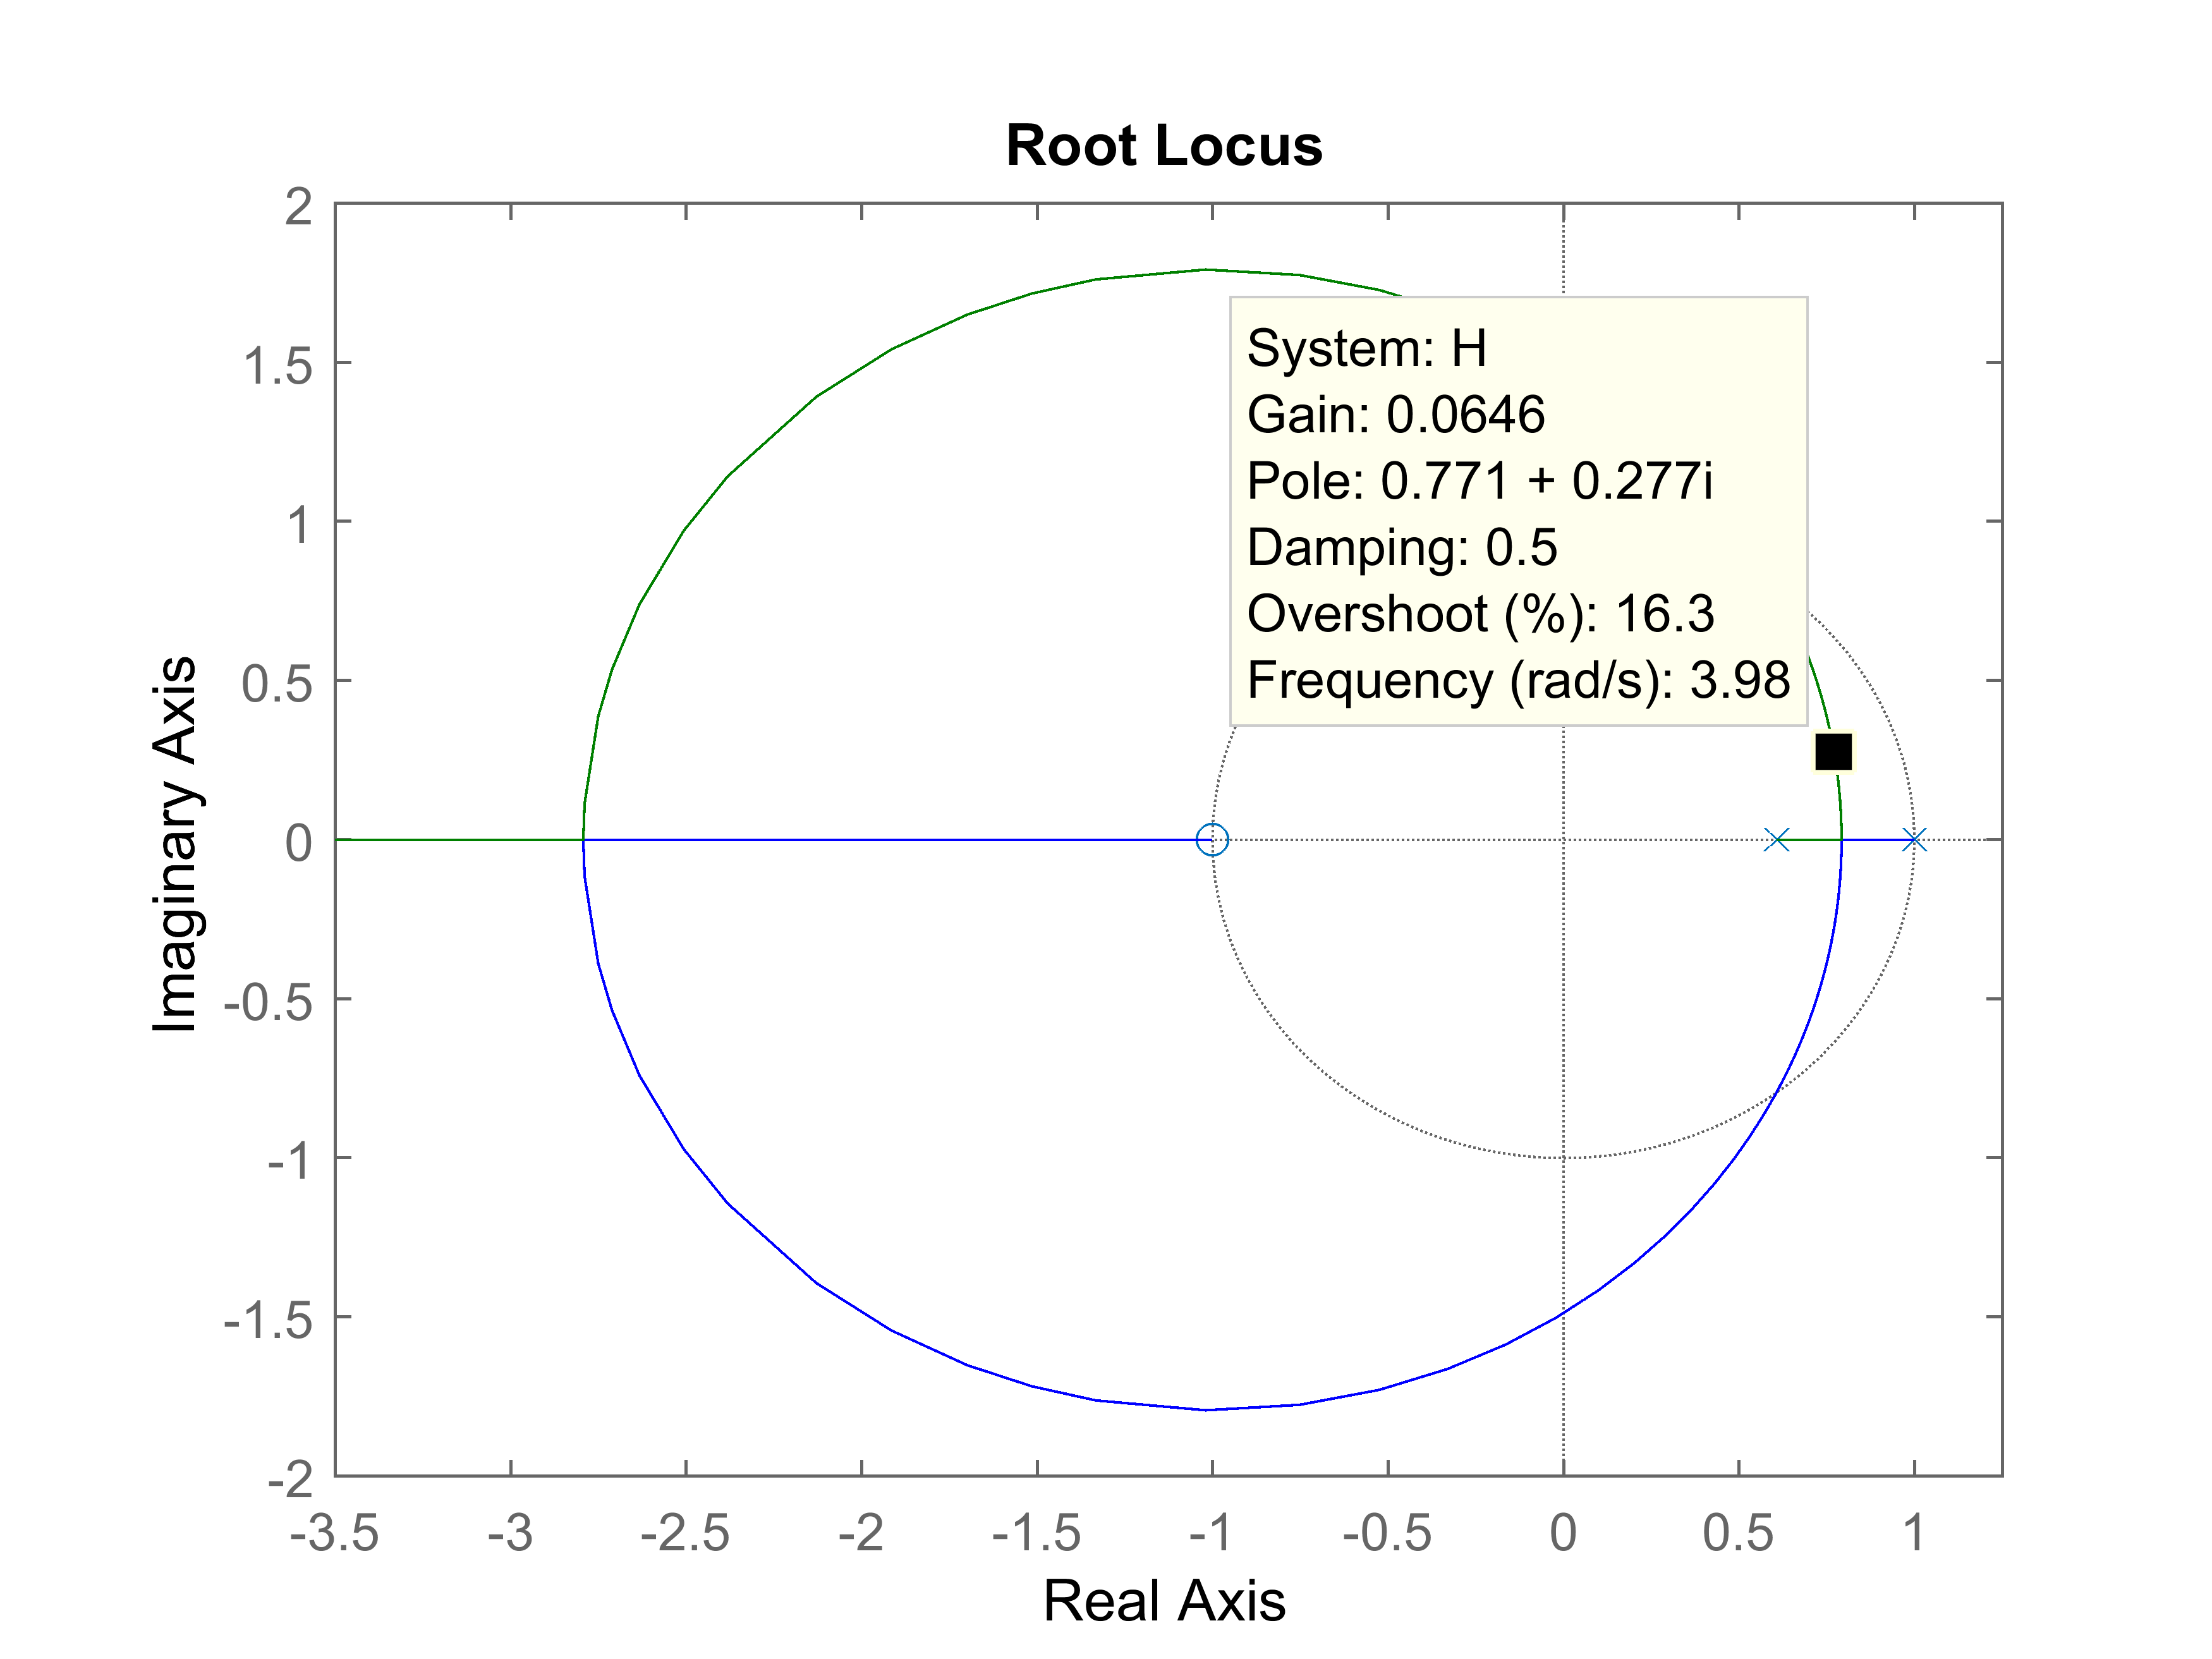
\includegraphics[width=1\linewidth]{Diagrams/B-4-8Rlocus2.png}
	\caption*{Root Locus For Figure 4-66}
	\label{fig:Rlocus}
\end{figure}
\end{minipage}
When $K=0.0646, \zeta=0.5$ with the pole at $z=0.771+j0.277=|0.8192|e^{j19.7620^\circ}$. 
\begin{align*}
z=  & |e^{-T(\zeta \omega_n)} |e^{T \omega_d} = |0.8192|e^{j19.7620^\circ} \\
& \omega_n = \frac{\ln(0.8192)}{(-0.1)(0.5)}=3.98854 = 4 \ \text{rad/s} \\
& \omega_d = \frac{(19.7629^\circ)}{0.1} = 3.449 \quad  \omega_d = \omega_n \sqrt{1-\zeta^2}=3.988 (0.866025)=3.4537 \ \text{rad/s} \\
& \text{Number of Samples per Cycle } = \frac{360^\circ}{T\omega_d}=\frac{360^\circ}{19.7629^\circ}=18.22
\end{align*}
	 %$P(z)=z^2-1.5419z+0.5419$, %$2 \zeta \omega_n =-1.5419$
%\begin{figure}[H]
%	\centering
%	\includegraphics[width=1\linewidth]{Diagrams/B4-8.pdf}
%	\caption*{Figure 4-66}
%	\label{fig:samplerblock48}
%\end{figure}


\subsubsection*{Problem B-4-12}
Design a digital proportional-plus-derivative controller for the plant whose transfer function is $1/s^2$, as shown in Figure 4-70. It is desired that the damping ratio $\zeta$ of the dominant closed-loop poles be 0.5 and the undamped natural frequency be 4 rad/sec. The sampling period is 0.1 sec, or $T=0.1$. After the controller is designed, determine the number of samples per cycle of damped sinusoidal oscillation.
\begin{figure}[H]
	\centering
	\includegraphics[width=1\linewidth]{Diagrams/block412.pdf}
	\caption*{Figure 4-70}
	\label{fig:blockB4-12}
\end{figure}
% https://www.wolframalpha.com/input/?i=inverse+laplace+transform+of+s
\vspace*{-1.05cm}
\begin{align*}
&  G_{PD}(s) = K_ds +K_p \quad G(z) = (1-z^{-1}) \mathcal{Z} \left\{\frac{1}{s^3} \right\} = \frac{(1-z^{-1})}{2} \mathcal{Z} \left\{\frac{2}{s^3} \right\} = \frac{(1-z^{-1})}{2} \frac{T^2z^{-1}(1+z^{-1})}{(1-z^{-1})^3} \\
& G_{PD}(z) =K_p+K_d(1-z^{-1})= (K_p+K_d)\cfrac{z-\frac{K_d}{K_p+K_d}}{z}, \quad G(z)=\frac{T^2z^{-1}(1+z^{-1})}{2(1-z^{-1})^2}=0.005\frac{(z+1)}{(z-1)^2} \\
& \omega_d = \omega_n \sqrt{1-\zeta^2} = 4 \sqrt{1-0.5^2}= 2 \sqrt{3} =3.4641 \ \text{rad/s}, \quad |z| = e^{T \zeta \omega_n} = e^{-T \zeta \omega_n} =e^{-0.2} = 0.8187 \\
& \angle z = \angle T \omega_d = 0.34641 \ \text{rad} =19.8478^\circ \quad  \text{Desired Pole } z = 0.8187 \angle 19.8478^\circ =0.7701+j0.2780 \\
& G_{PD}(z)G(z)= (K_p+K_d)\cfrac{z-\frac{K_d}{K_p+K_d}}{z}0.005\frac{(z+1)}{(z-1)^2}
\end{align*}

Computing the angle deficiency:
% https://www.wolframalpha.com/input/?i=1%2F(-0.2299%2Bi*0.2780)%5E2
% https://www.wolframalpha.com/input/?i=atan(0.2780%2F(0.7701-x))%2Bpi%3D0.500055555*pi
\begin{align*}
& % \left. \phase{\frac{1}{(z-1)^2}}\right \vert_{z=0.7701+j0.2780}
\phi_1=\phase{\frac{1}{(z-1)^2}} \bigg\vert_{z=0.7701+j0.2780} = \phase{\frac{1}{(-0.2299+j0.2780)^2}}= 100.82^\circ \quad \phi_2=\phase{z+1}\vert_{z=0.7701+j0.2780} =8.9255^\circ \\
& \phi_3 = \phase{\frac{1}{z}} \bigg\vert_{z=0.7701+j0.2780} =-19.84918^\circ \quad  \phi=180^\circ-\phi_1 -\phi_2-\phi_3=90.10^\circ \\
&\phi = \phase{z-\frac{K_d}{K_p+K_d}}\bigg\vert_{z=0.7701+j0.2780}=90.10^\circ \rightarrow \tan^{-1} \left({\cfrac{0.2780}{0.7701-\frac{K_d}{K_p+K_d}}} \right) + 180^\circ= 90.10^\circ \\
& \frac{K_d}{K_p+K_d} = 0.770149 \rightarrow G_{PD}(z)G(z)= (K_p+K_d)\cfrac{z-0.770149 }{z}0.005\frac{(z+1)}{(z-1)^2}
\end{align*}
\begin{align}
& \frac{K_d}{K_p+K_d} = 0.770149 \\
&\left|(K_p+K_d)\cfrac{z-0.770149 }{z}0.005\frac{(z+1)}{(z-1)^2} \right|\bigg\vert_{z=0.7701+j0.2780} =1
\end{align}
Solving for equations (1) and (2),

\[ 
K_p=9.833174968 \quad  K_d=32.9474741
\]

The controller $\displaystyle G_{PD}=42.7806\frac{z-0.770149}{z} = 42.7806(1-0.770149z^{-1})$. The number of cycles per second $n=\frac{360^\circ}{19.84918^\circ}=18.13678$
\end{document}

    
